\begin{tikzpicture}[
    >=Stealth,
    arrow/.style={->, thick},
    dashedbox/.style={
        draw,
        dashed,
        thick,
        rounded corners=4pt
    }
]

% ==================================================
% CAJA MODULADOR EMBEBIDO
% ==================================================

\node[dashedbox, minimum width=4cm, minimum height=4cm] (embeddedbox) at (-3,2.8)
{};

\node at (-3,5.2)
{
\small \textbf{Dispositivo Modulador}
};



% ==================================================
% CONTROLES ANALOGICOS
% ==================================================

\node (controls) at (-3,2.8)
{

\includegraphics[width=1.5cm]{fig/modulator.png}
};

\node[align=center] at (-3,3.8)
{
\scriptsize \textbf{Controladora}
};

% ==================================================
% CAJA SISTEMA EMBEBIDO
% ==================================================

\node[dashedbox, minimum width=10cm, minimum height=8.6cm] (embeddedbox) at (4.8,0.5)
{};

\node at (5,5.2)
{
\small \textbf{Sistema Embebido (Microcontrolador)}
};

% ==================================================
% GESTION DE ENTRADAS
% ==================================================

\node (inputs) at (1.3,2.8)
{

\includegraphics[width=1.4cm]{fig/input.png}
};

\node[align=center] at (1.3,3.7)
{
\scriptsize \textbf{Gestor de}\\[-7pt]
\scriptsize \textbf{entradas}
};

% ==================================================
% GENERADOR DE SEÑALES
% ==================================================

\node (generator) at (1.3,0)
{
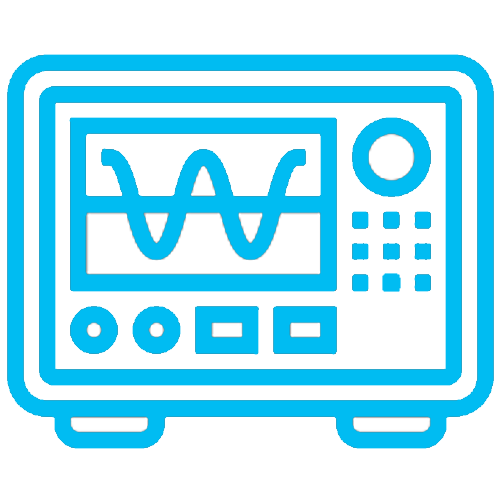
\includegraphics[width=1.4cm]{fig/signal.png}
};

\node[align=center] at (1.3,-0.9)
{
\scriptsize \textbf{Generador de}\\[-7pt]
\scriptsize \textbf{señales}
};

% ==================================================
% MODULO PROCESAMIENTO
% ==================================================

\node (processing) at (5.2,0)
{

\includegraphics[width=1.8cm]{fig/chip.png}
};

\node[align=center] at (5.2,1.3)
{
\scriptsize \textbf{Módulo de}\\[-7pt]
\scriptsize \textbf{Procesamiento}
};

% ==================================================
% ALGORITMOS
% ==================================================

\node (algorithms) at (5.2,-2.5)
{

\includegraphics[width=1.4cm]{fig/algorithm.png}
};

\node[align=center] at (5.2,-3.5)
{
\scriptsize \textbf{Algoritmos}
};

% ==================================================
% MODULO ENVIO
% ==================================================

\node (data) at (8,0)
{

\includegraphics[width=1.6cm]{fig/database.png}
};

\node[align=center] at (8,-1.1)
{
\scriptsize \textbf{Módulo de envío}\\[-7pt]
\scriptsize \textbf{de datos}
};

% ==================================================
% SERIAL
% ==================================================

\node (serial) at (11.2,0)
{

\includegraphics[width=1.5cm]{fig/serial.png}
};

\node[align=center] at (11.2,-0.9)
{
\scriptsize \textbf{Módulo de}\\[-7pt]
\scriptsize \textbf{transmisión serial}
};

% ==================================================
% APP BOX
% ==================================================

\node[dashedbox, minimum width=6cm, minimum height=6cm] (appbox) at (15.7,0.8)
{};

\node at (15.7,4.2)
{
\small \textbf{App de Monitoreo}
};

% ==================================================
% CONFIG
% ==================================================

\node (config) at (15,2.8)
{

\includegraphics[width=1.5cm]{fig/config.png}
};

\node[align=center] at (15,1.8)
{
\scriptsize \textbf{Módulo de }\\[-7pt]
\scriptsize \textbf{Configuración}
};

% ==================================================
% RX
% ==================================================

\node (rx) at (14.3,0)
{

\includegraphics[width=1.5cm]{fig/reconstruct.png}
};

\node[align=center] at (14.3,-1.2)
{
\scriptsize \textbf{Reconstrucción y}\\[-7pt]
\scriptsize \textbf{recepción de datos}
};

% ==================================================
% VISUALIZACION
% ==================================================

\node (visual) at (17,0)
{

\includegraphics[width=1.5cm]{fig/pc.png}
};

\node[align=center] at (17,-1.2)
{
\scriptsize \textbf{Módulo de}\\[-7pt]
\scriptsize \textbf{Visualización}
};

% ==================================================
% FLECHAS PRINCIPALES
% ==================================================

\draw[arrow] (controls.east) -- (inputs.west);

\draw[arrow] (inputs.south) -- (generator.north);

\draw[arrow] (generator.east) -- (processing.west);

\draw[arrow] (algorithms.north) -- (processing.south);

\draw[arrow] (processing.east) -- (data.west);

\draw[arrow] (data.east) -- (serial.west);

\draw[arrow] (serial.east) -- (rx.west);

\draw[arrow] (rx.east) -- (visual.west);

% ==================================================
% CONFIGURACION
% ==================================================
\draw[arrow] (config.west) -- (inputs.east);

\draw[arrow]
(visual.north)
|- (config.east);



\end{tikzpicture}